La visualización de datos es un área que tiene tiempo siendo explorada, donde el objetivo es lograr transmitir una información pero visualmente, es decir, mediante gráficas haciendo uso de colores, figuras, orientación, escalas, entre otros elementos. Es importante tomar en cuenta la visualización de datos en casos donde la información original a transmitir puede ser muy extensa y/o compleja, por lo tanto podemos hacerla más legible y comprensiva hacia una audiencia en específico. Posiblemente antes de representar la información visualmente esta tiene que ser transformada a otro tipo de dato dependiendo del caso. Es importante saber que existen dos paradigmas a la hora de realizar visualización de datos, explicativo y exploratorio \footnote{Exploratorio y explicativo \url{http://www.storytellingwithdata.com/blog/2014/04/exploratory-vs-explanatory-analysis}}.
\begin{itemize}
\item\textbf{Exploratorio}: cuando la audiencia/usuario está familiarizado con los datos y hace uso de la visualización para encontrar o formar algún patrón en particular.

\item\textbf{Explicativo}: cuando se quiere transmitir una información específica ya explorada hacia una audiencia que no tiene conocimiento alguno de los datos.
\end{itemize}
Para este trabajo especial de grado tenemos como meta una herramienta que ofrezca la posibilidad de construir gráficas en base a propiedades correspondientes a un historial de artículos de wikis, por lo tanto es indiscutible la necesidad de hacer uso de la visualización de datos. Cabe destacar que el historial de un artículo de wiki puede ser lo suficientemente extenso, por lo tanto representarlo de una forma visual, es decir, mediante algún tipo de gráfica, puede transmitir mejor una información que a simple vista no es obvia.

Construir una gráfica representativa puede llegar a tomarnos mucho tiempo y posiblemente ser compleja. La idea es aprovechar la existencia de avanzados proyectos que nos ayudan en la implementación de la visualización para facilitar el trabajo y de la misma forma, tener un mejor resultado. Existen muchas bibliotecas donde la mayoría tiene la misma finalidad, por lo que se realizó una búsqueda y evaluación, para luego quedar con las que mejores se adapten a las necesidades.

Para comenzar, hay que saber que las visualizaciones para este caso se construirán en el ámbito web, haciendo uso de HTML \cite{MozHTML} y JavaScript \cite{MozJS}. De las bibliotecas que nos apoyaremos, algunas construyen la gráfica utilizando el componente Canvas \cite{MozCanvas} de HTML5 y otras utilizando el estándar SVG \cite{W3SVG} (Scalable Vector Graphics).
\\[10pt]
\section[SVG vs Canvas]{SVG vs Canvas \cite{OperaSVGCanvas}}
El elemento Canvas es literalmente, un lienzo donde se va a pintar la gráfica, el proceso de construcción es más complejo y manual ya que la manera para dibujar consiste en pintar pixel por pixel, por lo que el cambio de resoluciones afecta lo dibujado. El elemento SVG (Scalable Vector Graphics) representa un vector escalable, donde cada elemento de la gráfica, ya sea una caja, círculo, texto, o imagen representa un sub-elemento del SVG general. Adicionalmente SVG permite el manejo de eventos y los cambios de resoluciones no afectan la visualización, esto hace que sea más fácil trabajar y personalizar los elementos de la gráfica a dibujar.

Como usaremos bibliotecas para la creación de las gráficas no debemos preocuparnos por la dificultad que toma la construcción con Canvas comparado con SVG, ya que la biblioteca lo hará por nosotros. El punto importante es que Canvas tiene un rendimiento mayor que el SVG cuando la gráfica maneja muchos objetos, debido a que cada objeto de la gráfica es un elemento que impacta en el DOM \cite{W3DOM} del HTML y esto hace que más memoria RAM sea consumida.
\\[20pt]
\section{Bibliotecas basadas en Canvas}
A continuación se presentará una lista de bibliotecas que construyen las gráficas haciendo uso de Canvas, acompañada de una lista de las gráficas principales que incluyen:
\\[10pt]
\begin{itemize}
\item\textbf{Processing.js\footnote{\url{http://processingjs.org/}}:}
Es un lenguaje de programación visual. Al ser un lenguaje de programación visual queda claro que su objetivo es general y no únicamente gráficas, por lo que nos permite elaborar desde animaciones hasta juegos. Basta con aprender sus definiciones propias para poder usarlo.
\item\textbf{Chartjs\footnote{\url{http://www.chartjs.org/}}:}
Biblioteca con aporte de 5 tipo de gráficas: gráfica de línea, barra, área polar, circular (dona), dispersión. En particular, las gráficas de esta biblioteca presentan un buen diseño adaptativo a distintos tipos de pantalla que pueden ser personalizado, incluyendo animaciones. Adicionalmente, podemos extender las funcionalidades descargando y configurando \textit{plugins} elaborados por otras personas.
\item\textbf{Echarts\footnote{\url{https://ecomfe.github.io/echarts-doc/public/en/index.html}}:}
Posee una gran variedad de gráficas personalizables y dando la posibilidad de habilitar animaciones. Ofrece soporte para la mayoría de los navegadores web y buena usabilidad para los dispositivos móviles, tanto rendimiento como adaptabilidad a la pantalla. La biblioteca con todas las gráficas y componentes incluidos ocupa alrededor de 500KB, pero es posible solo descargar algunos tipos de gráficas para reducir el tamaño de la biblioteca. Entre las gráficas disponibles se tienen: gráfica de línea, barra, área, mapa, circular (dona), dispersión, velas, grafos, boxplot, paralela, embudo y \textit{themeriver} (variación temática sobre el tiempo).
\\[15pt]
\end{itemize}
\section{Bibliotecas basadas en SVG}
A continuación se presentará una lista de bibliotecas que construyen las gráficas haciendo uso de SVG, acompañada de una lista de las gráficas principales que incluyen:
\\[10pt]
\begin{itemize}
\item\textbf{Raphael.js\footnote{\url{http://dmitrybaranovskiy.github.io/raphael/}}:}
Es una pequeña biblioteca \textit{cross-browser}, es decir, soportada por las mayoría de los navegadores web, con la capacidad de ofrecernos herramientas para elaborar cualquier visualización con vectores. No está orientada solo a la elaboración de gráficas, por lo que podemos crear cualquier visualización, ya sea juegos, alguna especie de arte o animación.
\item\textbf{Google Chart\footnote{\url{https://developers.google.com/chart/}}:}
Biblioteca elaborada por Google, donde ofrecen aproximadamente 29 tipos de gráficas, animadas, con un estilo minimalista y soporte para muchos navegadores, incluyendo versiones viejas. Además, nos permite configurar y personalizar las gráficas a nuestro gusto. La biblioteca solo ocupa 70 KB. Entre los tipos de gráficas disponibles destacan: gráfica de línea, barra, área, mapa, circular (dona), dispersión, intervalos, boxplot, velas, treemap y línea en el tiempo.
\item\textbf{Plotly.js\footnote{\url{https://github.com/plotly/plotly.js/}}:}
Es una biblioteca que está basada (construida) con ayuda de la biblioteca D3 y stackgl\footnote{Es un ecosistema para WebGL \url{http://stack.gl/}}. Tiene 20 tipos de gráficas, incluyendo en 3D (tres dimensiones) con un diseño agradable y con una cómoda caja de herramientas flotante para interactuar con la gráfica. Entre los tipos gráficas disponibles se tienen: gráfica de línea, barra, área, circular (dona), mapa, dispersión, boxplot, velas, treemap e histogramas (2D y 3D).
\\[15pt]
\end{itemize}
\section{D3 (Data-Driven Documents)}
D3 (Data-Driven Documents)\footnote{\url{https://d3js.org/}} es considerada una de las bibliotecas más potentes para la manipulación de datos, con varios años en desarrollo y con una comunidad bastante activa. Con esta biblioteca se puede llegar a construir casi cualquier tipo de gráfica deseable en SVG o HTML Canvas, gracias a que tenemos un control total sobre la construcción y diseño de la gráfica. También se dispone de \textit{plugins} y gran cantidad de ejemplos aportados por otras personas que pueden ayudarnos a facilitar la programación de la gráfica. La biblioteca tiene un tamaño base de 230 KB aproximadamente en su versión actual (v4.7.3).
Para hacer posible la construcción de una gráfica, D3 incluye los siguientes elementos claves:
\begin{itemize}
\item\textbf{Selecciones}: modificar elementos de manera imperativa, siendo menos tediosa a la tradicional.
\begin{lstlisting}
d3.selectAll("p").style("color", "white");
\end{lstlisting}
Podemos modificar atributos o estilos, registrar eventos, agregar, eliminar nodos logrando cambiar HTML o texto contenido.

\item\textbf{Propiedades dinámicas}: los estilos, atributos y otras propiedades pueden ser especificadas como funciones de datos, es decir no siempre reciben constantes.
\begin{lstlisting}
d3.selectAll("p").style("color", function() {
  return "hsl(" + Math.random() * 360 + ",100%,50%)";
});
\end{lstlisting}

\item\textbf{Entrar y salir}: facilita agregar y/o remover elementos en un grupo de datos.
\begin{lstlisting}
var p = d3.select("body")
  .selectAll("p")
  .data([4, 8, 15, 16, 23, 42])
    .text(function(d) { return d; });

// Entrar
p.enter().append("p")
    .text(function(d) { return d; });

// Salir
p.exit().remove();
\end{lstlisting}
En casos donde se busca optimizar esta sección es útil debido a que podemos establecer una navegación en la visualización y solo mostrar un grupo de elementos donde el resto se elimina, de tal forma que se vayan agregando y eliminando elementos a medida que se realicen acciones sobre la gráfica. 

\item\textbf{Transiciones}: existen controles para las animaciones, como la duración y tiempo de aplazo.
\begin{lstlisting}
d3.selectAll("circle").transition()
    .duration(750)
    .delay(function(d, i) { return i * 10; })
    .attr("r", function(d) { return Math.sqrt(d * scale); });
\end{lstlisting}
\end{itemize}
La biblioteca D3 no introduce una nueva representación visual como hace Raphael.js y Processing.js (bibliotecas mencionadas anteriormente), debido a que se trabaja directamente con estándares web (HTML, CSS \cite{MozCSS}, SVG), por ejemplo, podemos crear una gráfica en SVG y luego darle estilo con un archivo externo CSS. Sin embargo, estas tres (3) bibliotecas por el hecho de darnos una libertad total al construir visualizaciones requieren un tiempo considerado para aprender y poder usarlas debidamente.
\\[15pt]
\section{Evaluación de Bibliotecas}
Es importante saber que para nuestro caso todas las bibliotecas mencionadas anteriormente son las que mejor se adaptan según las necesidades, aún así se realizaron ciertas evaluaciones para decidir cuál utilizar. Para la evaluación se consideró lo siguiente:

\begin{itemize}
\item \textbf{Variedad de gráficas}

Para nuestro trabajo es necesario varios tipos de gráficas, ya que se realizarán visualizaciones con cantidad y tipo de datos distintos, por lo tanto es indispensable que existan diferentes tipos de gráficas para cada situación a visualizar en particular. Se revisó todos los tipos de gráficas que podían ofrecer cada una de las bibliotecas. Si es necesario un diseño o tipo de gráfica bastante particular probablemente para ese caso la mejor opción sería D3, Raphael.js o Processing.js.

\item \textbf{Rendimiento}

Definimos rendimiento como el comportamiento que toma la biblioteca al construir una gráfica considerablemente pesada (con inmensa cantidad de datos). El problema que podemos presentar al visualizar grandes cantidades de datos es que la vista donde está la gráfica se perciba con cierta lentitud y en el peor de los casos el navegador (browser) se detenga, es decir deje de trabajar. Afortunadamente, hay algunas bibliotecas que optimizan las gráfica y aplican un estilo de paginación, donde no dibujan todos los puntos a la vez, sino a medida que nos profundizamos en la gráfica.

Se sometieron algunas de las bibliotecas a la creación de una gráfica desde 10.000 hasta 1.000.000 de datos. En la \textbf{Figura \ref{fig:library_comparison}} podemos apreciar una aproximación del resultado basado en la cantidad de objetos que pudieron soportar, en donde el eje 'y' corresponde al número de objetos, donde M representa el millón. Cabe destacar que D3, Processing y Raphael no fueron considerados ya que su rendimiento es totalmente relativo a como se programe la gráfica.
\bigbreak
\begin{center}
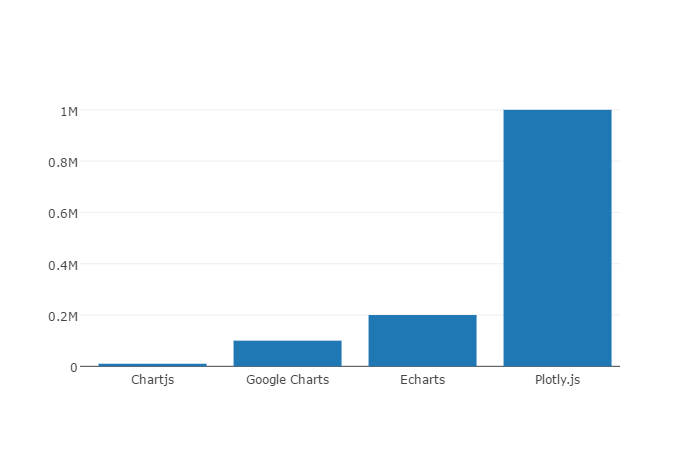
\includegraphics[scale=0.45]{library_comparison.png}
\captionof{figure}{Comparación de bibliotecas de visualización}
\label{fig:library_comparison}
\end{center}
\bigbreak
\end{itemize}
Al finalizar la evaluación, quedamos con tres (3) candidatos: D3, Echarts y Plotly. Donde cada uno predomina en distintos escenarios necesarios para nuestro trabajo. Adicionalmente, \textbf{D3} al ser una biblioteca que nos ofrece la mayor libertad para elaborar gráficas a nuestro gusto dará aquel soporte en gráficas sumamente específicas, también viene acompañada de muchos ejemplos elaborados por la comunidad que pueden servir de apoyo. \textbf{Plotly} a pesar de construir las visualizaciones en SVG logra un excelente rendimiento, aún mejor que el resto de las bibliotecas, además su diseño es agradable y nos ofrece una caja de herramientas para interactuar con la gráfica. Como último candidato a \textbf{Echarts}, por su gran variedad de ejemplos y los posibles tipos de gráficas que nos puede ofrecer, agregando que, dan soporte con gráficas que son usables en dispositivos móviles logrando además un buen rendimiento para aquellos sistemas de bajos recursos.











